\documentclass[12pt]{article}
\usepackage{enumitem}
%\usepackage[T1]{fontenc}
\usepackage[auth-sc,affil-sl]{authblk}
\usepackage{amsmath}
\usepackage{graphicx}
\usepackage{color}
\usepackage[toc,page]{appendix}
%\usepackage{enumerate}
\usepackage[round]{natbib}
%\usepackage{url} % not crucial - just used below for the URL 
%\usepackage{amsthm}
\usepackage{amssymb}
\usepackage{graphicx}
\usepackage{epstopdf}
\usepackage{hyperref}
\usepackage{alltt}
\usepackage{listings}
\usepackage{array}
\usepackage[noline, boxed, linesnumbered, procnumbered, titlenumbered]{algorithm2e}
%\usepackage[firstpage]{draftwatermark}
\usepackage[margin=1in]{geometry}  %%jcgs has own margins
\usepackage{lmodern}
\usepackage{caption}
\usepackage{subcaption}

%\pdfminorversion=4
% NOTE: To produce blinded version, replace "0" with "1" below.
\newcommand{\blind}{0}

\newcommand{\secref}[1]{Section~\ref{#1}}
\newcommand{\appdxref}[1]{Appendix~\ref{#1}}
\newcommand{\tblref}[1]{Table~\ref{#1}}
\newcommand{\figref}[1]{Figure~\ref{#1}}
\newcommand{\thmref}[1]{Theorem~\ref{#1}}
\newcommand{\algref}[1]{Algorithm~\ref{#1}}
\newcommand{\funref}[1]{Function~\ref{#1}}
\newcommand{\listingref}[1]{Listing~\ref{#1}}

\newcommand{\eg}{{\em e.g.}}
\newcommand{\ith}{$i^{th}$}
\newcommand{\cut}[1]{}
\newcommand{\todo}[1]{{{\color{red}{[#1]}}}}

\newcommand{\Ex}{\mathop{\mathbb{E}}}
\newcommand{\Imp}{\mathbf{I}}

\newcommand{\spd}{\fontfamily{cmr}\textsc{\small StratPD}}
\newcommand{\cspd}{\fontfamily{cmr}\textsc{\small CatStratPD}}
\newcommand{\xnc}{$x_{\overline{c}}$}
\renewcommand{\xi}{x^{(i)}}
\newcommand{\xnC}{$x_{\overline{C}}$}

\setlist[enumerate]{itemsep=-1mm}

% DON'T change margins - should be 1 inch all around.
\cut{
\addtolength{\oddsidemargin}{-.5in}%
\addtolength{\evensidemargin}{-.5in}%
\addtolength{\textwidth}{1in}%
\addtolength{\textheight}{1.3in}%
\addtolength{\topmargin}{-.8in}%
}

\begin{document}

\def\spacingset#1{\renewcommand{\baselinestretch}%
{#1}\small\normalsize} \spacingset{1}


%%%%%%%%%%%%%%%%%%%%%%%%%%%%%%%%%%%%%%%%%%%%%%%%%%%%%%%%%%%%%%%%%%%%%%%%%%%%%%

\if0\blind
{
  \title{\bf Tech Report: Model-Free Feature Importances}

  \author{Terence Parr and James D. Wilson\\
      University of San Francisco\\
}
  \maketitle
} \fi

\if1\blind
{
  \bigskip
  \bigskip
  \bigskip
  \begin{center}
    {\LARGE\bf Title}
\end{center}
  \medskip
} \fi

\bigskip
\begin{abstract}
dsf
\end{abstract}

\noindent%
{\it Keywords:} feature importance, partial dependence, model interpretability, machine learning
%\vfill

%\newpage
%\spacingset{1.5} % DON'T change the spacing!
\section{Introduction}
\label{sec:intro}

\todo{wrapper vs filter methods}

Among data analysis techniques, feature importance is one of the most  useful. Data science practitioners use feature importance to gain business insights (e.g., identifying product characteristics valued by customers) and to select features for predictive models (dropping the least predictive features to simplify and potentially increase the generality of the model). While some approaches work directly on the data, such as principle component analysis (PCA) or minimal-redundancy-maximal-relevance (mRMR) by \cite{mRMR}, almost all feature importance algorithms analyze data through interrogation of a specific  fitted model (SHAP, permutation, drop column), or even interrogating subsidiary models to analyze such fitted models (LIME).

But, relying on a fitted model is problematic. Practitioners must choose an appropriate model that captures the relationship between features and target. Inaccurate models do not yield useful feature importance results, yet, there is no definition of ``accurate enough.'' More importantly, it is possible to get very different feature importances running the same algorithm on the same data, just by choosing a different model. Feature importances derived from a model indicate how well that specific model is able to take advantage of the features, rather than the predictiveness or importance intrinsic to those features of the data.  This fact is troubling and calls into question the validity of importances derived from imperfect models using any technique.  

Consider the feature importance graphs in \figref{fig:diff-models} derived from four different models on the same, well-known Boston toy data set, as computed by SHAP \cite{shap} that has recently emerged as the front runner in feature importance. The linear model (a) struggles to capture the relationship between features and target ($R^2$=0.74), so those importances should not be trusted.  In contrast, the random forest (b), boosted trees (c), and support vector machine (d) models capture the relationship in the training records (all 506) with high fidelity, but SHAP derives meaningfully different feature importances from each model.  This is particularly true given the high variance of the importances computed from the random forest. \todo{explain that} It is unclear which results, if any, are correct. (If humans could examine the data directly to find the true feature importances, we would not need feature importance algorithms.) (we'll intro fitness measure in \secref{foo}.)

\begin{figure}[htbp]
\begin{center}
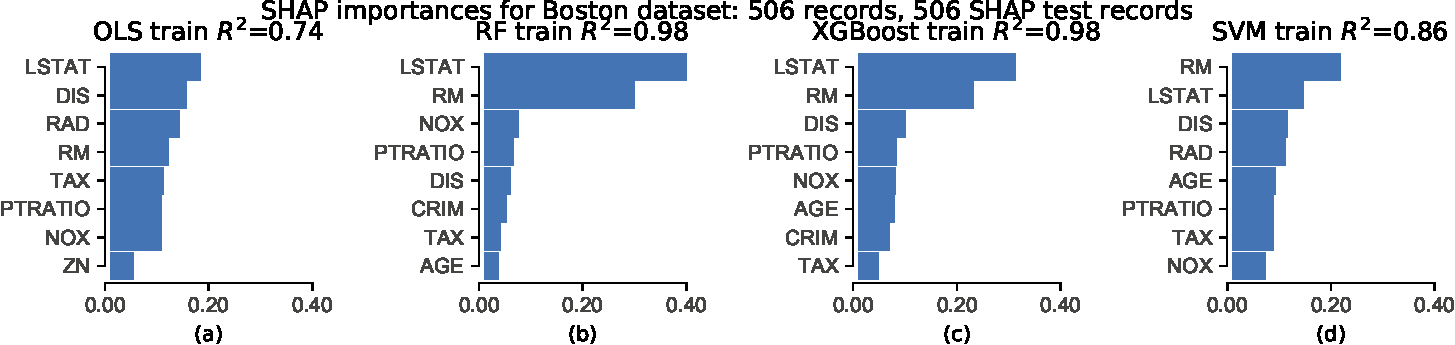
\includegraphics[scale=0.6]{images/diff-models.pdf}
\caption{Top 8 of 13 features. {\tt\footnotesize RandomForestRegressor(n\_estimators=30)}, {\tt\footnotesize XGBRegressor(max\_depth=5, eta=0.01, n\_estimators=50)}, {\tt\footnotesize SVR(gamma=0.001, C=100)} High var for RF. nshap=n test records. Rough timing for explaining 506 test records is (a) less than 1 second, (b) 10s, (c) 3s, and (d) 50s.}
\label{fig:diff-models}
\end{center}
\end{figure}

The differences clearly arise because the feature importances are distorted by the lens' of the models. Current techniques peer through the model (and possibly through an extra, explanatory model) to the underlying data, but true feature importances are relationships that exist in the data, with or without a model.  For example, to gain business insights about customers, a predictive model is unnecessary and a data analysis technique that revealed importances directly from the data would be sufficient and preferable. \todo{maybe say PCA does this although limited to linear features and assumes most spread = most important?} Besides, predictive features do not always coincide with important features; e.g., some models are unable to capture nonlinear relationships and, therefore, always find them non-predictive.  \todo{last bit redundant?}
 
In our experience, it is best to get importances using multiple techniques and to view the combined results as a clue rather than the gospel truth.  The unfortunate reality, though, is that practitioners routinely make business decisions and  perform feature selection using the results provided by machine learning libraries without questioning their validity.  For example, \cite{rfpimp} demonstrated that the widely-used {\em gini-drop} technique, specific to random forests and provided by the popular {\tt scikit-learn} Python library, gives inappropriate weight to features with many unique values, even pure noise features. (The gini-drop of a feature is the average drop in gini impurity for decision nodes splitting on that feature.) \todo{transition}

Despite many years of research attention, there is still no widely-accepted definition of feature importance. While there are multiple precisely-defined algorithms with known strengths and weaknesses, all interrogate fitted models for predictions. The primary contributions of this paper are (1) a simple, intuitive definition of feature importance that operates purely on the training data without making predictions from a model and (2) an implementation that yields plausible and effective results, as measured by the {\em top-k} fitness metric defined in \secref{sec:experiments}.

~\\
\noindent \todo{Likely a good spot for a paper walk-through}

\section{A definition of feature importance}\label{sec:def}

Practitioners loosely define feature importance as measuring feature predictiveness, which presupposes a fitted predictive model, probably because importances are so often used for feature selection during model development.  Research  focuses on more accurately identifying the impact of features upon model predictions.  But, relying on a fitted model makes it difficult to tease apart the true feature importance from the ability of the model to exploit that feature for prediction purposes. Rather than measuring feature impact on {\em model predictions}, we propose avoiding the model completely to define feature importance as the average impact of a feature on the {\em data set response values}.

Assume we are given training data pair ($\bf X, y$) where ${\bf X} = [x^{(1)}, \ldots, x^{(n)}]$ is an $n \times p$ matrix whose $p$ columns represent observed features and ${\bf y}$ is the $n \times 1$ vector of responses. In special circumstances, we know the precise importance of each feature $x_j$.  For example, if a data set is generated using a linear function, $y = \beta_0 + \sum_{j=1}^p \beta_j x_j$, \todo{assumes independence of $x_j$?} then coefficient $\beta_j$ corresponds exactly to the importance of $x_j$.  $\beta_j$ is the impact on $y$ for a unit change in $x_j$, holding all other features constant.

To hold features constant for more general functions, we can take the partial derivatives of $y$ with respect to each feature $x_j$. Imagine there exists a smooth function $f:\mathbb{R}^{p} \rightarrow \mathbb{R}$ that precisely maps each $\xi$ to $y_i$, ${y_i} = f(\xi)$. \todo{should that be $y^{(i)}$ to be consistent?} The partial derivative of $y$ with respect to $x_j$ gives the change in $y$ holding all other variables constant; e.g., for linear functions, $\beta_j = \frac{\partial y}{\partial x_j}$. Integrating the partial derivative then gives the {\em partial dependence}  of $y$ on $x_j$, the isolated contribution of $x_j$ to $y$. But, rather than relying on a fitted model as originally formulated by \cite{PDP}, this definition of partial dependence relies on the partial derivative of a known function that generated the data set.

~\\
\noindent {\bf Definition 1} The partial dependence of $y$ on feature $x_j$ evaluated at $x_j = z$ is the cumulative sum up to $z$:

\begin{equation}\label{eq:pd}
\text{\it PD}_j(z) = \int_{min(x_j)}^z \frac{\partial y}{\partial x_j} dx_j
\end{equation}

$PD_j(z)$ is the value contributed to $y$ by $x_j$ at $x_j = z$ and, at the left edge of the curve, $PD_j(0)=0$. The advantage of this partial dependence definition is that it is insensitive to collinear or otherwise codependent features, unlike the traditional definition that is most accurate for models ``{\em dominated by low order interactions}'' per Friedman.  To go from partial dependence to feature importance, we compare the area under each partial dependence curve. The larger the area under the curve, the larger the impact on $y$.

~\\
\noindent {\bf Definition 2} The feature importance of $x_j$ is the expected value of the absolute value of $x_j$'s partial dependence: $\Imp_j = \Ex[|\text{\it PD}_j|]$. Or, normalized to be in [0,1]:

\begin{equation}\label{eq:Epd2}
\Imp_j = \frac{\Ex[|\text{\it PD}_j|]}{\sum_{k=1}^p \Ex[|\text{\it PD}_k|]}
\end{equation}

The mean value theorem of integrals implies that the area under a curve in interval $[a,b]$ is equal to the average function value times the range $b-a$.  Because we are evaluating each partial dependence curve at exactly $N$ points per feature, the ``mass'' under each curve has the same range factor:

\[
\Imp_j = \Ex[|\text{\it PD}_j|] (max(x_j) -min(x_j)) \frac{N}{(max(x_j) -min(x_j))} = \Ex[|\text{\it PD}_j|] N
\]

\todo{say we normalized so they are comparable; normalized to N not arbitrary $x_j$ range, or just say that we normalize to 0..1 without loss of generality; same as multiplying by that factor}

\noindent The $N$ range factor is the same for each importance, so for comparison purposes it drops out.  On a given data set, the expectation is just the average ($N_j$ is the number of unique $x_j$ values):

\begin{equation}\label{eq:Epd}
\Ex[|\text{\it PD}_j|] = \frac{1}{N_j} \sum_{i=1}^{N_j} |\text{\it PD}_j(x_j^{(i)})|
\end{equation}

\noindent The feature importance of $x_j$ is then just how much, on average, $x_j$ pushes $y$ away from zero.   As an example, consider quadratic equation:

\begin{equation}\label{eq:quad}
y = x_1^2 + x_2 + 100
\end{equation}

\noindent as a generator of data for $x_j \sim U(0,3)$. The partial derivatives are $\frac{\partial y}{\partial x_1} = 2 x_1$ and $\frac{\partial y}{\partial x_2} = 1$, giving $\text{\it PD}_1 = x_1^2$ and $\text{\it PD}_2 = x_2$. The areas under the partial dependence curves in $[0,3]$ are $\Imp_1 = \frac{x_1^3}{3} \big |_0^3 = 9$ and $\Imp_2 = \frac{x_2^2}{2} \big |_0^3 = 4.5$.   Therefore, $x_1$ is twice as important as $x_2$ for data generated in that interval with normalized importances $\Imp_1 = 0.\overline{66}$ and $\Imp_2 = 0.\overline{33}$.

The obvious disadvantage of this feature importance definition is that function $f$ is unknown in practice, so symbolically computing the partial derivatives is not a viable approach. But, if we could compute exact partial dependence curves by some other method, then this definition would be still be a viable approach to get true feature importances. While partial dependence curves derived from fitted models, as originally defined, are biased in the presence of codependent variables, we introduced a technique called \spd{} (\cite{stratpd}) to approximate unbiased partial dependence curves using a data stratification approach, rather than through a fitted model. \todo{In a nutshell, \spd{} ...}

\section{Related work}

 these are not comparable but as they have the same goal and are the primary means to obtain future importance now, we summarize existing techniques.

PCA is in a new space and so impossible to interpret and not able to really give us feature order but we can approximate by using the ``loads'' associated with the first principal component.

 relevance: how correlated in the general sense is a feature with the response variable?
 
 redundancy:  how much information is shared with codependent features. this can be computed using multicollinearity (RF trained on all but $x_j$ to predict $x_j$.
 
 feature selection proceeds by ordering features by most to least relevant. 
 
Pearson but limited to linear.

Spearman ranked correlation  for monotonic relationship

 could use mutual information here as well ( expensive?)
 
 both ignore co-dependencies; so two identical features will appear side-by-side in the ranking, even though one should be tossed out.

Instead of picking the first/top $k$, use a greedy selection algorithm to balance relevance with redundancy.

redundant variables are a problem because selection repeatedly selects features with much the same relationship or effect upon the response variable.

\todo{We deal with all possible combinations for codependency's because of the nature of the partial dependence mechanism.}

Relief Algorithm \cite{relief} limited to 2 class problems. \cite{ReliefF}  those multiclass problems. apparently does not deal with redundancy but does deal with interactions. RReliefF works for regression. \cite{RReliefF}. Idea is to weight weight features by how well they distinguish between classes by repeatedly sampling from the data set and updating weights according to the distance between near miss (diff class) and near hit (same class).

 classification only. minimal-redundancy-maximal-relevance (mRMR) by \cite{mRMR}  takes correlation-width, output a step further to deemphasize codependent features. greedy algorithm selects features one by one to minimize a loss func.  measuring relevance and redundancy.  works only on classification as formulated. it's unclear how you would measure the correlation between a categorical that was label encoded and a numerical column. what about correlation of two categoricals? correlation implies order but nominal categorical variables are not ordered. they use F statistic between numerical and target labels and then Pearson between numerical features. somebody claims that it does not deal with interactions nor non-pairwise collinearity. does it rely on density estimates? mRMR  at each step it selects the future with maximum value of relevance - average pairwise redundancy with other features. \todo{should we bother putting in the equation?}
 
 for more see survey \cite{survey}

Existing techniques are variations on a single theme: tweak the model by adding/subtracting/permuting features and measuring the impact on model accuracy (permutation and drop column) or average response (SHAP). LIME has a linear model that approximates the output in a neighborhood of x for each x.

Here is where we show that SHAP gets $y = x_1^2 + x_2 + 100$ wrong.

\section{Experimental results}\label{sec:experiments}

\todo{an experiment where we show and sensitive to noise column}

\todo{maybe show the linear 1 1 1 codependence example}

\todo{what about outlier example}

\todo{stability is valuable. users would not trust results that changed significantly for small data set changes. show our error bars from bootstrapping and say we can do p-values.}

\todo{bulldozer: YearMade ignores too much with stratpd, use catstrat}

Even with domain expertise, humans are unreliable estimates of feature importance. Otherwise, we would need feature important mechanisms. Comparing the quality of feature importance methods is then a challenge. The simplest approach is to compare methods on synthetic data for which the answer is clear, such as the quadratic in \ref{eq:quad}.

For real data sets, we can train a predictive model on the most important $k$ features and compare prediction error. The importance method that accurately identifies the most impactful features without getting confused by codependent features, should yield lower production errors for a given $k$.   This mirrors how one would use it for model feature selection.
 
The best feature importance method ranks features by their independent contributions to $y$, without getting confused by codependent features. The most important single feature as reported by two importance methods can be used to train a model and measure a prediction metric.
 
{\bf Definition 3} The {\em top-k} fitness measure trains a suitable model on the  most important $k$ features as reported by two or more importance methods then compares prediction metrics. Actually p246 \cite{liu-fs} has an example of this.

even if recommendations are identified by their isolated contribution, the model is still taking the combination into consideration when fitting and hence the marginal errors are not necessarily reduced specifically because of the added feature at number $k$.

Get a baseline \figref{fig:baseline}.

\begin{figure}[b]
\centering
\begin{subfigure}{.5\textwidth}
    \centering
\includegraphics[scale=0.7]{images/rent-topk-spearman.pdf}
\vspace{-2mm}\subcaption{\footnotesize foo}\vspace{3mm}
\end{subfigure}%
\begin{subfigure}{.5\textwidth}
    \centering
\includegraphics[scale=0.7]{images/bulldozer-topk-spearman.pdf}
\vspace{-2mm}\subcaption{\footnotesize foo}\vspace{3mm}
\end{subfigure}
\caption{Whew}
\label{fig:baseline}
\end{figure}

Model-based methods have all the advantages in these experiments.

In \figref{fig:features}, we

Then see \figref{fig:topk}

\begin{figure}[b]
\centering
\begin{subfigure}{.5\textwidth}
    \centering
\includegraphics[scale=0.7]{images/boston-topk.pdf}
\vspace{-2mm}\subcaption{\footnotesize foo}\vspace{3mm}
\end{subfigure}%
\begin{subfigure}{.5\textwidth}
    \centering
\includegraphics[scale=0.7]{images/flights-topk.pdf}
\vspace{-2mm}\subcaption{\footnotesize foo}\vspace{3mm}
\end{subfigure}
\begin{subfigure}{.5\textwidth}
    \centering
\includegraphics[scale=0.7]{images/bulldozer-topk.pdf}
\vspace{-2mm}\subcaption{\footnotesize foo}\vspace{3mm}
\end{subfigure}%
\begin{subfigure}{.5\textwidth}
    \centering
\includegraphics[scale=0.7]{images/rent-topk.pdf}
\vspace{-2mm}\subcaption{\footnotesize foo}\vspace{3mm}
\end{subfigure}
\caption[short]{A beautiful, well written caption}
\label{fig:topk}
\end{figure}

\begin{figure}[b]
\centering
\begin{subfigure}{1\textwidth}
    \centering
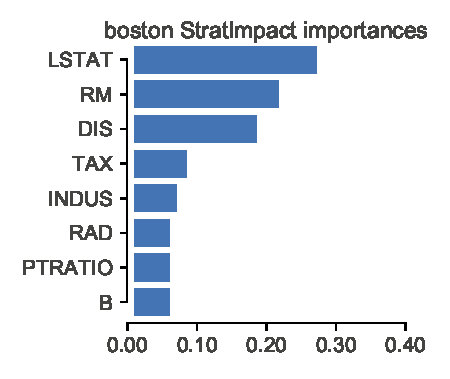
\includegraphics[scale=0.6]{images/boston-features.pdf}
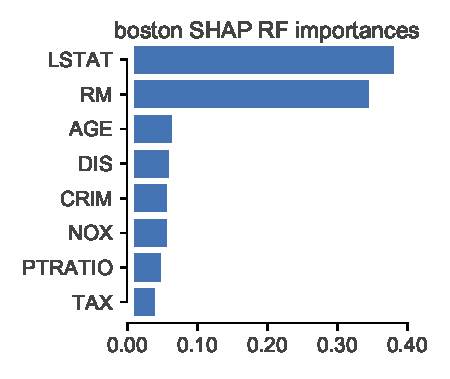
\includegraphics[scale=0.6]{images/boston-features-shap-rf.pdf}
\vspace{-2mm}\subcaption{\footnotesize Note LSTAT/RM order is diff than in original figure as their is high variance}\vspace{3mm}
\end{subfigure}%
\hfill
\begin{subfigure}{1\textwidth}
    \centering
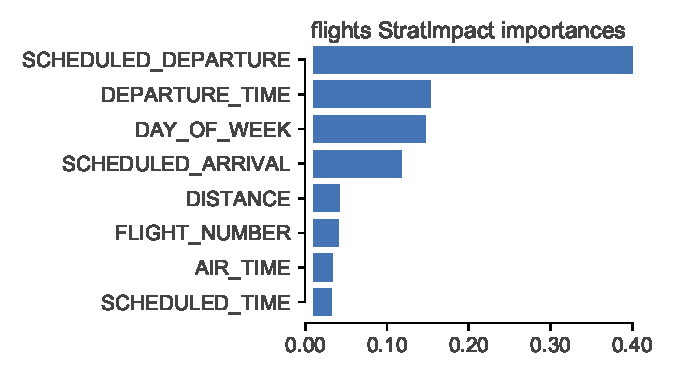
\includegraphics[scale=0.6]{images/flights-features.pdf}
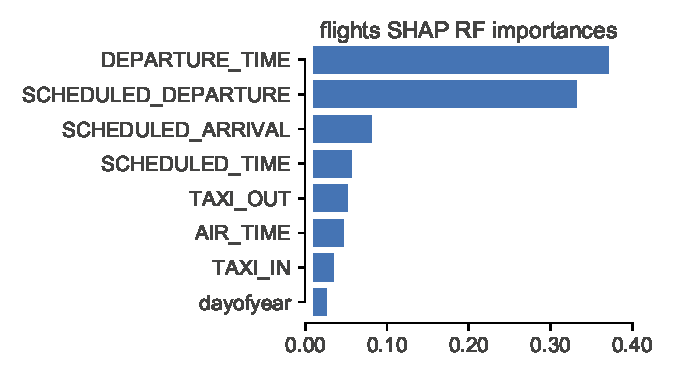
\includegraphics[scale=0.6]{images/flights-features-shap-rf.pdf}
\vspace{-2mm}\subcaption{\footnotesize 5.8M records}\vspace{3mm}
\end{subfigure}
\hfill
\begin{subfigure}{1\textwidth}
    \centering
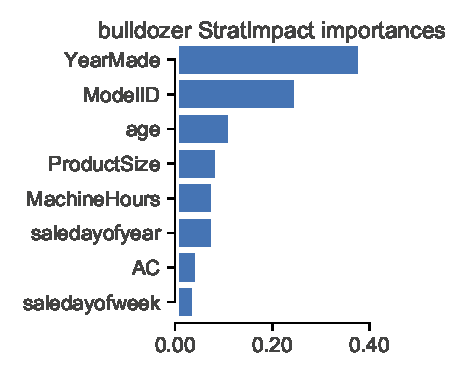
\includegraphics[scale=0.6]{images/bulldozer-features.pdf}
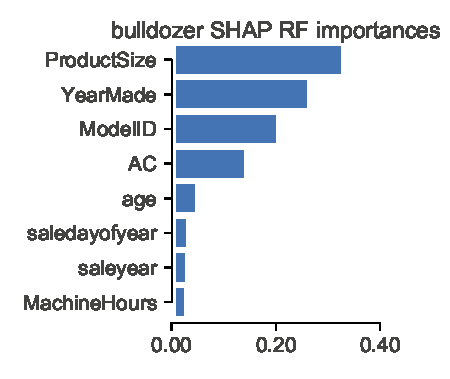
\includegraphics[scale=0.6]{images/bulldozer-features-shap-rf.pdf}
\vspace{-2mm}\subcaption{\footnotesize foo}\vspace{3mm}
\end{subfigure}%
\hfill
\begin{subfigure}{1\textwidth}
    \centering
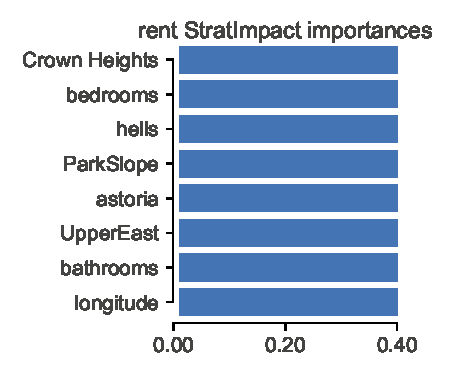
\includegraphics[scale=0.6]{images/rent-features.pdf}
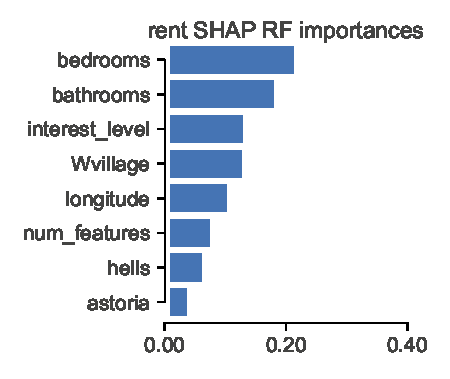
\includegraphics[scale=0.6]{images/rent-features-shap-rf.pdf}
\vspace{-2mm}\subcaption{\footnotesize foo}\vspace{3mm}
\end{subfigure}
\caption[short]{blorttttt}
\label{fig:features}
\end{figure}


Consider the recommendations from OLS SHAP used in a random forest. In general, they are not good recommendations. This demonstrates that the rank of features is highly dependent upon the model used to get those recommendations. In some cases, plain OLS recommendations fitted to RF beats the recommendations from OLS SHAP fitted to the RF.

Do an experiment that compares PCA and Spearman's R against StratImpact.

performance. with lots of outliers, choosing a small subset for shap is a bad idea so this is a real problem. linear and boosted trees are efficient but RF are not and I wouldn't consider anything using the general explainer.

There are issues surrounding how many explanatory samples you can use. 300 even run a couple of times is not enough to sample 5.8M records.
 
\section{foo}

 what is the definition: loosely as which are most predictive

The variance of the importances derived from the random forest is high, SHAP has specialized ``explainers'' for linear and tree-based models for performance reasons, but relies on the general method to explain support vector machines. , but the results are subject to the variance of the internal model parameters.  Ideally, feature importances would not change from run to run on the same data set using the same technique.

\section{Discussion and future work}

research should now focus on getting more accurate partial dependence approximations.

must define for classification

\bibliographystyle{apalike}

\bibliography{pdimp}
\end{document}